\documentclass[border=8pt]{standalone}
\usepackage[T1]{fontenc}
\usepackage{lmodern}
\usepackage{tikz}
\usetikzlibrary{arrows.meta,calc}
\renewcommand{\familydefault}{\sfdefault}
\definecolor{left}{HTML}{1F4E9A}
\definecolor{right}{HTML}{B5306B}
\definecolor{mid}{HTML}{333333}
\begin{document}
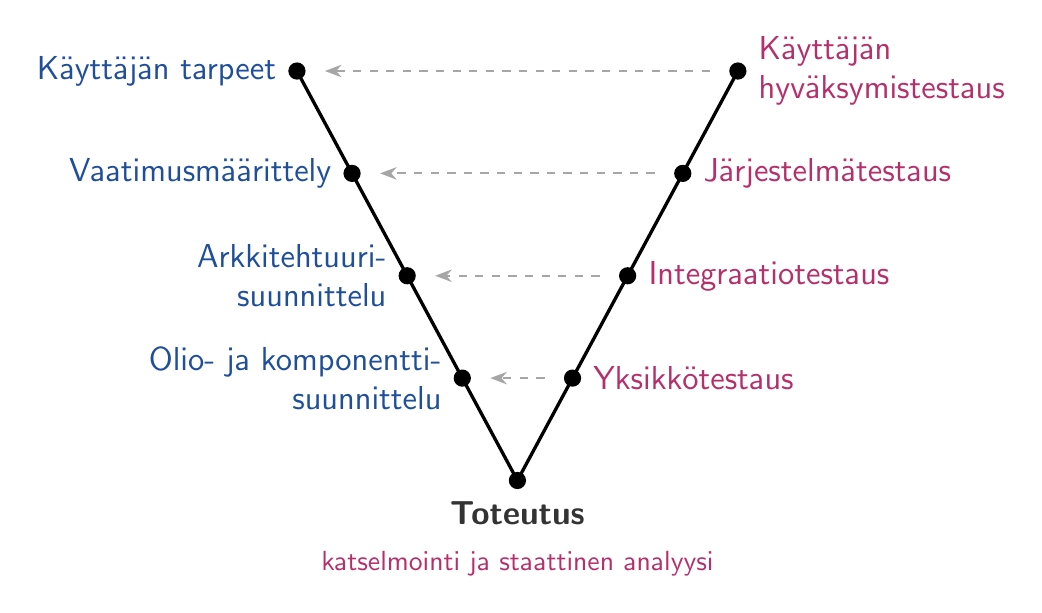
\begin{tikzpicture}[
  dot/.style={circle,fill=black,inner sep=2.2pt},
  L/.style={left,text=left,font=\large,align=right,xshift=-4pt},
  R/.style={right,text=right,font=\large,align=left,xshift=4pt},
  link/.style={shorten >=3pt,shorten <=3pt,dashed,gray!70,-{Stealth[length=6pt]},thick}
]
% V points: levels y=4,3,2,1, bottom 0
\foreach \y/\n in {4/a,3/b,2/c,1/d}{
  \coordinate (L\n) at ({-0.7*\y},{1.3*\y});
  \coordinate (R\n) at ({0.7*\y},{1.3*\y});
}
\coordinate (B) at (0,0);
\draw[very thick] (La) -- (Ld) -- (B) -- (Rd) -- (Ra);
\foreach \n in {a,b,c,d}{ \node[dot] at (L\n){}; \node[dot] at (R\n){}; }
\node[dot] at (B){};
\node[L] at (La) {Käyttäjän tarpeet};
\node[L] at (Lb) {Vaatimusmäärittely};
\node[L] at (Lc) {Arkkitehtuuri-\\suunnittelu};
\node[L] at (Ld) {Olio- ja komponentti-\\suunnittelu};
\node[R] at (Ra) {Käyttäjän\\hyväksymistestaus};
\node[R] at (Rb) {Järjestelmätestaus};
\node[R] at (Rc) {Integraatiotestaus};
\node[R] at (Rd) {Yksikkötestaus};
\node[below=4pt,text=mid,font=\large\bfseries,align=center] at (B) {Toteutus};
\node[below=22pt,text=right,font=\normalsize,align=center] at (B) {katselmointi ja staattinen analyysi};
\foreach \n in {a,b,c,d}{ \draw[link] ($(R\n)+(-0.25,0)$) -- ($(L\n)+(0.25,0)$); }
\end{tikzpicture}
\end{document}
